%!TEX root = ../thesis.tex
%*******************************************************************************
%*********************************** First Chapter *****************************
%*******************************************************************************


\chapter{Introduction and literature review}


\ifpdf
    \graphicspath{{Chapter1/Figs/Raster/}{Chapter1/Figs/PDF/}{Chapter1/Figs/}}
\else
    \graphicspath{{Chapter1/Figs/Vector/}{Chapter1/Figs/}}
\fi

%*******************************************************************************


\section[Motivation for research and historical background]{Motivation for research and historical background}
\label{section1.1}

\subsection[History of early modern English wall paintings]{History of early modern English vernacular wall paintings}
\label{subsection1.1.1}

From the mid 1500s to early 1600s, elaborate and bold wall paintings were fashionable and popular around England and Wales across all classes with disposable income.~\autocite{Baird_thesis,Davies_book,Kirkham_thesis} Two recent comprehensive studies have been carried out, by Kirkham in Suffolk and Norfolk and by Baird/Davies in the Welsh Marches. Although this trend was shortlived, it is significant because it appeared during a period of other significant changes in English society. There was increased social mobility, increasing numbers of lower gentry and well established merchant classes, and as a result there was uncertainty and instability in defining class and status.~\autocite{Baird_thesis} 

Architecturally, the Great Rebuilding caused dramatic changes to how people lived. Historians observe a movement away from the Medieval open hall to houses with smaller rooms with specific purposes and greater privacy.~\autocite{Baird_thesis,Davies_book,Hamling_book} The Reformation and resulting iconoclasm led to destruction of religious images in churches, a critical source of visual vocabulary for most of society, and restricted the subjects considered ideologically acceptable in secular buildings as well.~\autocite{Kirkham_thesis,Hamling_book,Giles} Finally, trade with the continent and printing press allowed dissemination of images thus trends from elite society down to the normies. While it is beyond the scope of this work to discuss these social changes in detail, they are important for contextualizing wall paintings. Furthermore, wall paintings offer a rare view into the choices and fashions of the middling class during a period of upheaval.~\autocite{Kirkham_thesis,Baird_thesis}

Wall paintings during this period were characterized by a wide range of quality and aesthetic appeal, especially to the 21st century viewer. Floral/foliate motifs as well as antiquework style designs originating from Italy and arabesques originating from Islamic designs were widely used.~\autocite{Kirkham_thesis,Baird_thesis,Thornton_book} Fewer figurative and religious subjects were observed, particularly in Suffolk, though these subjects are noted in Baird/Davies' study of the Welsh Marches. Many wall paintings imitated textiles and wood panelling, both unaffordable for middling folk. 

Finally, many paintings incorporated texts into imitation textiles or with decorative borders.~\autocite{Baird_thesis,Kirkham_thesis} Texts were often placed over fireplaces or over doors, and were used to teach morals as part of the maintenance of a Godly Protestant household.~\autocite{Hamling_book} Many paintings do not survive due to destruction or overpainting, and have been neglected in spite of the information they contain about how social status was communicated and gained, and how people conceived of the home.~\autocite{Benton1,Benton2,Kirkham_thesis}

The cost of wall painting schemes depended on the cost of materials such as pigments as well as labor cost; the extent of the scheme and the skill required to lay out the pattern.~\autocite{Baird_thesis,Davies_book,Kirkham_thesis} Pigments were also chosen, beyond cost, for their aesthetic effect.~\autocite{Kirkham_thesis} Some patrons chose more muted colors, using, for instance, umber or red and yellow earth pigments. Others chose brighter, flashier pigments such as vibrant orpiment yellow or blue verditer. 

Kirkham suggests that blue verditer may have been selected because it was a newly available, fashionable pigment. It was often used in urban schemes in Suffolk rather than in rural areas, and has not been found in the Welsh Marches to date.~\autocite{Kirkham_thesis,Baird_thesis} This may be due to availability related to commerce links with London and the continent but also could be due to local trends. Blue rooms were quite fashionable at the time, influenced by French court styles, and the presence of a blue room in an early modern house was a marker of elite status or aspirations.~\autocite{Kirkham_thesis}

\subsection[Historical use of blue pigments in wall paintings]{Historical use of blue pigments in wall paintings}
\label{subsection1.1.2}

The use of blue pigments during this period is of specific interest due to their limited availability and high cost. There were four blue pigments available to vernacular painters - indigo/woad (diff plant same chemical), blue verditer, smalt, and azurite. Azurite was not widely observed at the vernacular level, and ultramarine was not used at any level for decorate plainting due to its rarity and cost.~\autocite{Kirkham_thesis} While only indigo/woad were observed in the Welsh Marches, blue verditer and (rarely) azurite were observed in the East of England.~\autocite{Baird_thesis,Davies_book,Kirkham_thesis} Smalt, a blue-coloured crushed glass, was difficult to work with and not used extensively.~\autocite{Kirkham_thesis}

Azurite is a naturally occurring basic copper carbonate with the chemical formula Cu\textsubscript{3}(CO\textsubscript{3})\textsubscript{2}(OH)\textsubscript{2}.~\autocite{Aru,Smieska} It forms around copper deposits and was mined during this period in eastern Europe, with important mines in Hungary and Germany.~\autocite{Aru} It has been used throughout history, and is observed in Egyptian art as well as Medieval European works, particularly in illuminated manuscripts.~\autocite{Smieska} Seldes et. al. identified azurite in several fine art works from South America painted during the 1700s, and determined that the pigment was referred to by Spanish artists as ``blue powder" or ``blue ashes."~\autocite{Seldes} Clarke et. al. have also identified azurite in 13th century Japanese scroll paintings.~\autocite{Clarke} Many other mineral impurities are commonly observed in natural azurite formations, and these as well as variations in the size of particles affects the color and visual effect of the pigment.~\autocite{Smieska,Price,Cardell}

Blue verditer is the synthetic analog of azurite and has been identified in wall paintings dating to the early 1600s (1610-1620 as earliest approximate date of use). In Kirkham's study of wall paintings in Suffolk country, she finds blue verditer in several of the more elaborate decorative schemes as well as in the inventories of painters, merchants, and grocers. The cost of blue verditer depended on the quality, and was slightly below indigo and several times less expensive than the cheapest grade of azurite.~\autocite{Kirkham_thesis} 

Blue verditer was made as a by-product of gold refining, but was challenging to produce to high quality standards. Further study of the sources of historical verditer has not been carried out, though Kirkham suggests the Netherlands as a possible source.~\autocite{Kirkham_thesis,Kirby} Identification of artificial blue and green pigments by scientific methods has not been widely undertaken. Naumova et. al.'s studies of Russian frescoes is one example of extensive analysis, but does not employ recent advances in chemical analysis.~\autocite{Naumova1994,Naumova1990} This work is discussed further below.

Many recipes purporting to produce blue and green copper-based pigments synthetically exist dating back to Greek artists as well as the medieval period.~\autocite{mappae_clavicula,Orna_literature,Orna_silver,Barnett} Orna et. al. have discussed and evaluated medieval recipes claiming to produce blue pigment from the treatment of silver and copper metals. Treatment of copper containing alloys with acetic acid under different heating conditions formed verdigris and copper acetate, but copper carbonates were not observed.~\autocite{Orna_literature,Orna_silver}

MacTaggart et. al. studied recipes for producing blue and green verditer, which are the synthetic analogues of azurite and malachite. Blue verditer is also referred to as ``blue bice" and ``blue ashes." They discuss previously identified characteristics of historic verditers, ``tiny, rounded, fibrous aggregates, even in size, highly birefracting, and blue by transmitted light." There are credible historical references to verditers dating to the early 1500s, and they claim that blue verditer was a speciality of English producers at this time. One challenge, however, is that the authors note that blue verditer was also used as a general term to refer to any blue pigments at the time regardless of composition or production. 

In order to determine a successful method for producing verditers that meet previously identified physical markers, they tested the procedure for refining gold for which blue verditer was a byproduct. Ultimately, they struggled to produce blue verditer consistently, as did early modern refiners, and they proposed that the success or failure of synthesis was dependent on the weather; blue particles are only produced at temperatures below 12 \textdegree C.~\autocite{MacTaggart}
%- color dependence on grain size - smieska, painting manuals, that other ref about separating the sizes, cardell, price

\subsection[Open research questions about wall paintings]{Open research questions about wall paintings and early modern material culture}
\label{subsection1.1.3}

While there are many aspects of early modern material culture that are not well understood today, including the extent and significance of wall paintings created in the early modern period, this research is concerned with the open questions relating to the materiality of these works. There has been limited research into the materials used by craftsmen due to the difficulty of carrying out scientific analysis on a large number of samples.~\autocite{Baird_thesis, Davies_book} The availability of various blue (and, to a lesser extent, green) pigments during this period has been subject to debate, and the language used to describe blue pigments has been inconsistent and scientifically inaccurate.~\autocite{Harley} 

In particular, the use of synthetic copper carbonate blue pigments (blue verditer) has been noted in Suffolk.~\autocite{Baird_thesis, Kirkham_thesis} This discovery must be corroborated and a larger body of samples should be analyzed to determine the extent of use. This is significant to the interpretation of vernacular wall paintings, particularly their purpose, cost, value to homeowner, and disposability.~\autocite{Baird_thesis,Davies_book} Additionally, the availability of synthetically produced pigments to the middling class could indicate new industrial methods of production and close ties between scientists and the artists and craftsmen who they supplied. 

This work also has important implications for preservation and restoration of these works, which are often in poor condition or at risk of being lost entirely. Many vernacular wall paintings from this period exist in the historical record but have since been demolished, although experts on early modern material culture maintain their importance to our understanding of daily life during the period.~\autocite{Davies_book,Hamling_book,Benton1,Benton2} Azurite and verditer pigments are unstable and can be altered by excessive humidity and alkalinity, as well as light exposure, and this research could inform future preservation and restoration choices made about these important works.~\autocite{Saunders,Cardell,Lluveras,Mattei,Dei}

\section[Research plan and scientific background]{Research plan and scientific background}
\label{section1.2}

\subsection[Plan for sampling and analysis]{Plan for sampling and analysis}
\label{subsection1.2.1}

\todo{Reiterate: unanswered questions are primarily 1) the identity of pigments used in wall paintings in Suffolk (XXXX check, how big range of sampling is) and 2) the method of production of these pigments, including the determination of viability of synthetic recipes from the time.

Note methods that we intend to use (AFM IR, Raman, SEM-EDS, microscopy..?). What information these will give, and how this information will be useful in answering the above questions.

Explain samples that will be analysed- the sources, locations, why these were selected. This cannot be completed yet, but the reference samples can be discussed at this point.}

\subsection[Previous work on copper carbonate pigments]{Previous work on copper carbonate pigments}
\label{subsection1.2.2}

Previous work has characterised azurite and malachite and degradation products thereof using confocal Raman spectroscopy and infrared specroscopy. The use of and production of synthetic blue and green pigments in England and continental Europe has been minimally studied. Additionally, synthetic recipes from the medieval period have been evaluated for their success in producing pigments.

Frost et. al. have studied malachite and azurite using confocal and polarised Raman spectroscopy, giving a clear explanation of peak assignments and determining that these minerals do show orientation dependence in their spectra.~\autocite{Frost} Bicchieri et. al. used micro-Raman and laser indused breakdown spectroscopies to study lapis lazuli and azurite pigments on parchment.~\autocite{Bicchieri} 

Saunders et. al. have studied the changes azurite undergoes upon exposure to high humidity, noting that azurite has been observed to degrade to malachite or green copper chlorides under various environmental conditions. They found that azurite was largely unaffected by light under all humidity conditions, with one sample forming copper chlorides in the presence of NaCl and one inexplicably darkening.~\autocite{Saunders} Cardell et. al., on the other hand, determined that azurite was altered by natural (outdoor) and artificial ultraviolet light exposure, showing that effects were dependent on pigment grain size.~\autocite{Cardell} Lluveras et. al. mapped green degradation products using synchrotron radiation, determining that copper oxalates and copper hydroxychlorides formed in different areas of the azurite surface depending on proximity to calcium and chlorine ions respectively.~\autocite{Lluveras} The chemical heterogeneity observed here supports the use of surface analytic techniques such as AFM-IR. 

Mattei et. al. addressed the degradation of azurite induced by exposure to heat and exposure to alkaline conditions. They note that azurite is not very stable, degrading easily to form malachite, to Cu2Cl(OH)3 (atacamite, paratacamite or clinoatacamite), or less often to CuS or CuO (tenorite). They note a green inclusion present in azurite samples that was not malachite or a yellow iron oxide. Tenorite was found following heating of azurite particles, and degradation is dependent on the size of the pigment grain. Tenorite was also found following exposure to alkaline terra cotta. Beyond this, however, they did not discuss alterations to crystal structure and did not measure the depth of penetration into the sample.~\autocite{Mattei} 

Naumova et. al. have studied the green pigments used in medieval Russian frescoes dating to the 1500s, and have identified several synthetic pigments for which recipes from the period are not known. They note that artificial pigments were typically circular in grain shape and showed a characteristic black cross when viewed under a polarised microscope through crossed nicol prisms. However, these identifiers are noted in the same work to be problematic and inaccurate at times. Naumova et. al. also attempted to recreate historic recipes for blue and green pigments, and were unable to synthetically produce azurite. This is one of few sources that does discuss the use of synthetic pigments, and concludes that further research is necessary in this area.~\autocite{Naumova1994,Naumova1990}

Aru et. al. have characterised the mineral impurities present in many samples of azurite from source mines known in the medieval period using Raman spectroscopy. Many minerals were discovered as natural inclusions in most samples, including malachite, hematite, goethite, cuprite, and titanium dioxides. Others were less common, such as quartz, calcite, cerussite, orthoclase, beudantite and jarosite. Tenorite, identified by XXXX et. al. as a degradation product of azurite, was not identified as an impurity in these samples. Unfortunately, though the samples were collected from mines that were active during the medieval period, they dated at the earliest to the eighteenth century, and the small sample size precludes the use of impurities to conclusively trace provenance of azurite samples.~\autocite{Aru} However, this research does suggest that the presence of trace minerals in natural samples is indicative of environmental conditions when azurite crystals form, and that these minerals should be studied in a larger sample set to determine whether any patterns in their occurrence can be identified. This supports the use of techniques that detect surface heterogeneity and suggests that mineral inclusions may differ in natural versus artificial samples.

\todo{Remaining to do: All the things I havent read yet!!!

Dei - degradation products

Gunn - Chemical Reactions between Copper Pigments and Oleoresinous Media, pigment interactions

Linke - The detection of copper-based pigment darkening by biuret-reaction in mural paintings by SEM-EDX, micro-XRF and micro-Raman spectroscopy

Odlyha - Dosimetry of paintings: Determination of the degree of chemical change in museum exposed test paintings (smalt tempera) by thermal analysis

Scott - A Review of Copper Chlorides and Related Salts in Bronze Corrosion and as Painting Pigments

CURRENT: Smieska - Trace elements in natural azurite pigments found in illuminated manuscript leaves investigated by synchrotron x-ray fluorescence and diffraction mapping}


\section[Methodology and theoretical background]{Methodology and theoretical background}
\label{section1.2}

\todo{SEM, EDS, etc}

\subsection[Confocal Raman spectroscopy]{Confocal Raman spectroscopy}
\label{subsection1.2.2}

Raman spectroscopy uses the interactions between photons from an incident laser beam and molecules or particles in the sample to identify functional groups and other molecular structures present. Incident photons at a specific frequency with energy $E_{in} = h\nu$ are directed at the surface of the sample, where they scatter back and are detected. Most photons are scattered back at the same energy, undergoing elastic collisions; this is known as Rayleigh scattering. Some, though, return at higher energies (Anti-Stokes scattering) or lower energies (Stokes scattering). In the case of Stokes scattering, which is the scatter detected for analysis:

\begin{equation} \label{eq:raman_1}
E_{out} = E_{in} - \Delta E
\end{equation}

with $E_{out}$ as the energy of the photon that returns from the sample surface. Stokes scattering is more common than Anti-Stokes scattering because the vast majority of sample molecules are in their ground vibrational state at room temperature. This means that they do not have excess vibrational energy to transfer to the incident photon. $\Delta E$ is the change in energy between the ground ($E_{g}$) and excited ($E_{ex}$) vibrational states:

\begin{equation} \label{eq:raman_2}
\Delta E = E_{ex} - E_{g}
\end{equation}

This change in energy $\Delta E$ is known as the Raman shift. Different bonds have different vibrational modes so they also have different Raman shifts, and the Raman shift is also affected by the chemical environment of the bond. This means that the technique can identify not only different molecules and compounds in a sample, since they each produce a distinct Raman spectrum, but also chemical and structural changes.~\autocite{2018RS,horiba,matousek_tissue} Changing chemical environments induce shifts in peak centers as well as broadening. Relative peak intensities can indicate degrees of disorder or the loss of specific types of bonds or functional groups.~\autocite{tomasini_raman}

The selection rules for a bond to be Raman active require perturbation of the polarisability (or transient dipole) of the molecule. This means that, unlike infrared spectroscopy, Raman spectroscopy is capable of detecting symmetric vibrational modes.~\autocite{2018RS,inphotonics}

Raman spectroscopy is widely used in conservation science. Analysis does not necessarily damage or destroy samples, and it is capable of informing scientists about both inorganic materials such as many pigments and organic materials such as binders and other pigments.~\autocite{conti_2016} Raman spectroscopy has been used to study many pigments and binders, to identify chemical species, and monitor changes due to ageing and environmental exposure as well as pigment-binder interactions.~\autocite{conti_2016,matousek_tissue,tomasini_raman,pallipurath2014,pallipurath2013,lazzari,vandenabeele} 

\subsection[Atomic force microscopy]{Atomic force microscopy}
\label{subsection1.2.2}

Atomic force microscopy (AFM) coupled to infrared spectroscopy is an exciting novel analytic method for studying surfaces below the diffraction limit.~\autocite{dazzi2017,kurouski} It has been used previously to study artworks and heritage objects. Latour et. al. studied the degradation of collaged in historic parchments, Morsch et. al. have investigated heterogeneity of epoxy surfaces as well as linseed oil interactions with titanium dioxide pigment, and Ma et. al. studied the formation of metal carboxylate salts in oil paint.~\autocite{latour,Morsch,morsch2016,ma} Most significantly, AFM-IR has only microdestructive sampling requirements and provides a great deal of information about the physical and chemical properties of surfaces.~\autocite{dazzi2017,kurouski}

Conventional infrared spectroscopy has an inherent resolution limit related to the wavelength of incident light; the diffraction limit for an incident beam of $\lambda$ is $\lambda$/2. Typically, this is approximately several hundred nanometers to several microns. AFM, on the other hand, uses a narrow physical probe to investigate properties of the sample instead. This means that the resolution is limited to the size of the probe, and can be as small as sub-20 nm.~\autocite{dazzi2017} In addition to studying the friction, roughness, and topography of the sample surface using physical probe-surface interactions, recent work has coupled the high resolution of AFM to infrared spectroscopy providing information about chemistry of the surface.~\autocite{dazzi2017,kurouski}

When the AFM probe interacts with the surface, the cantilever is deflected and, like a spring, oscillates. A laser that is reflected off the cantilever into a detector registers the oscillation. Images can be collected in tapping mode, where the probe is not constantly in contact with the surface, or in contact mode where the tip moves along the surface maintaining the interaction. Surface friction is measured using the side-to-side deflection of the tip in contact mode.~\autocite{friction_afm} Infrared spectra are collected by measuring the probe displacement due to thermal expansion of the sample, caused by incoming infrared radiation.~\autocite{dazzi2017,kurouski} The infrared collection system is shown in \textit{Figure \ref{fig:afm_diagram}}.

\mynote{Is it okay to reuse figures from mphil that I made?}

\begin{figure}[H]
\centering
  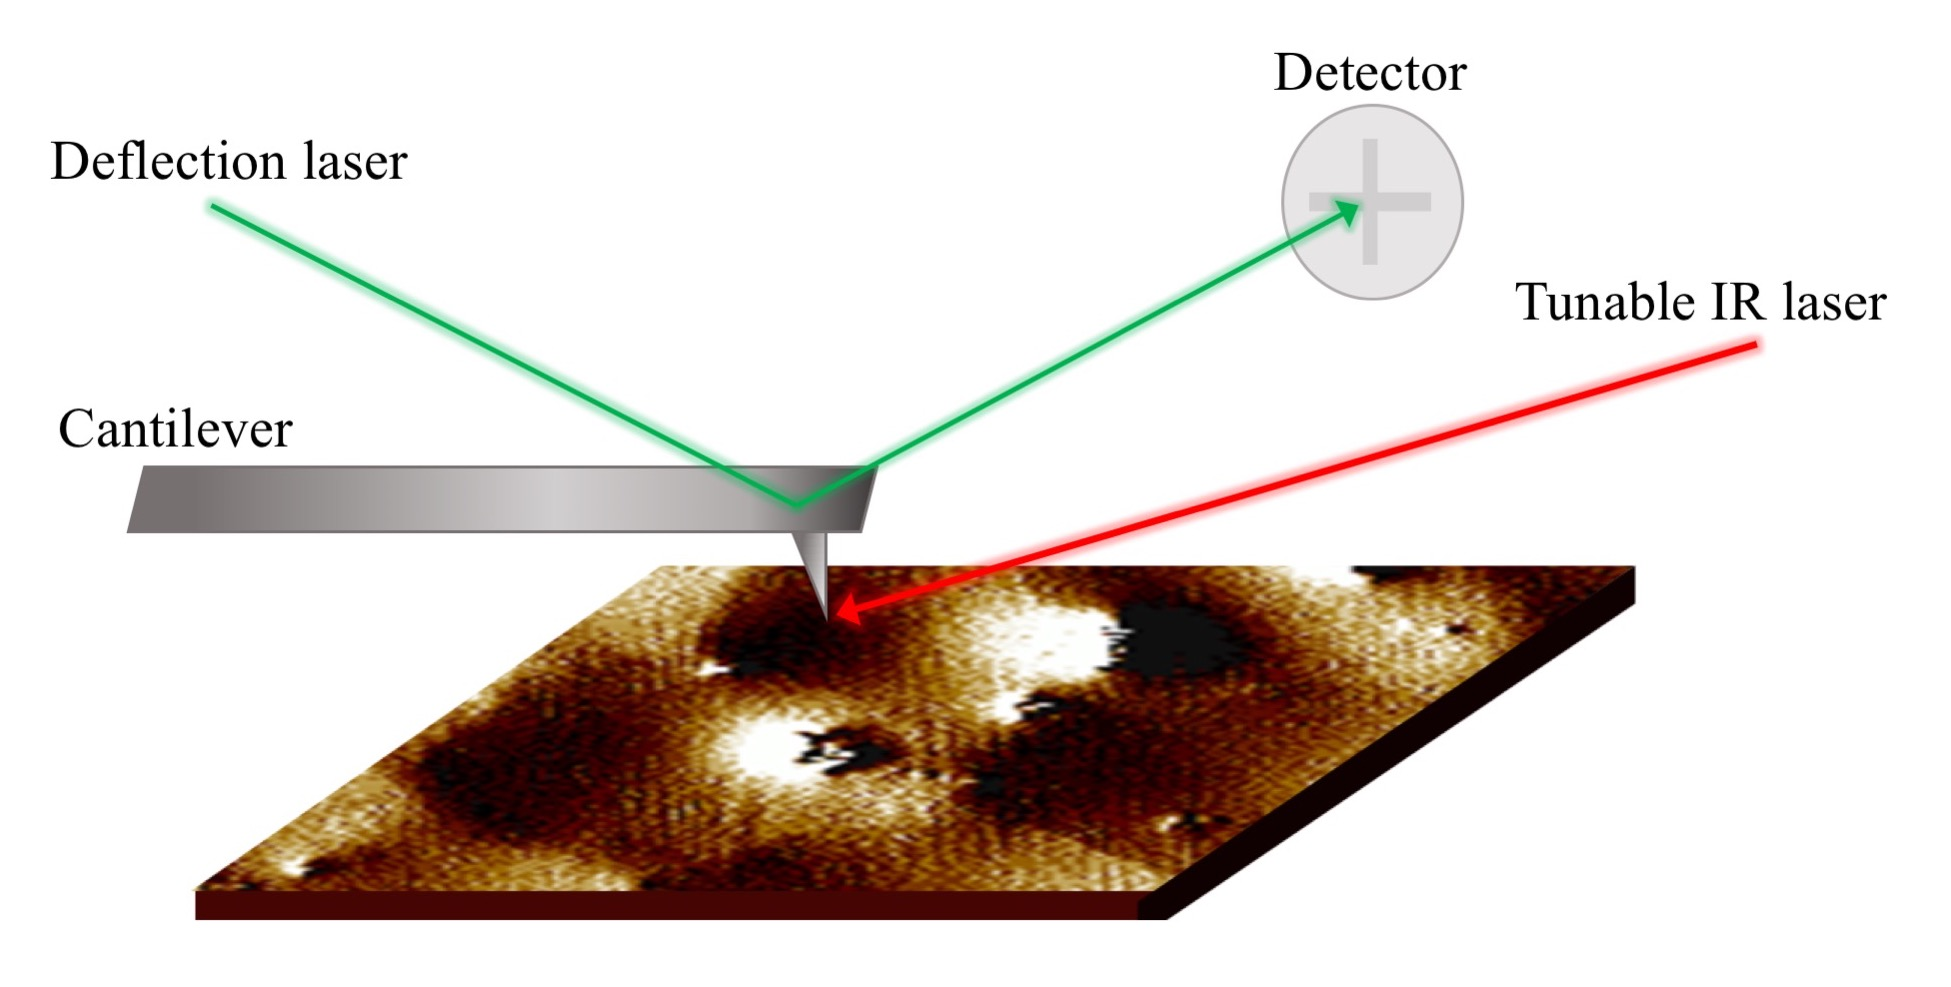
\includegraphics[width=\linewidth]{afm_diagram}
\caption[Diagram of AFM-IR schematic showing a top-down illumination system.]{Diagram of AFM-IR schematic showing a top-down illumination system. The incident inrared beam causes the sample to expand and move the probe-cantilever system. The cantilever deflection is recorded and detected by another laser beam reflected into a photodiode detector.~\autocite{Morsch,dazzi2017}}
\label{fig:afm_diagram}
\end{figure}

AFM-IR spectra are directly comparable to conventional IR spectra because the oscillations of the cantilever are proportional to the absorption coefficient of the sample. This means that peak locations and band shapes will not be affected by the collection method, and samples can be studied using both methods concurrently.~\autocite{dazzi2017,kurouski} It is possible to collect either at one point on the sample over all frequencies, generating a spectrum, or over all points on the sample at a single frequency, generating a map of the intensity at that frequency. 

\subsection[Scanning electron microscopy]{Scanning electron microscopy}
\label{subsection1.2.2}

 \todo{Needs writing.}



